\chapter{Evaluación y selección de modelos}\label{Chapter4} 
% chktex-file 8
% chktex-file 12
% chktex-file 13
% chktex-file 44

Cualquier método de aprendizaje estadístico sufre en situaciones de pocos datos de entrenamiento y alta dimensionalidad de entrada. Además, una parte clave es la estandarización de los datos (predictores y variable/s dependiente/s); si bien hay métodos en los que no es necesario estandarizar alguna de estas, es recomendable hacerlo. \\
\begin{equation}
x \to \frac{x - \bar{x}}{\text{std}x} = x'
\end{equation}
    
Al estandarizar una variable $x$ a $x'$, la media de $x'$ es 0 y la desviación estándar 1. Si se ha estandarizado la variable dependiente, es necesario desestandarizar la salida, así como su error y desviación estándar (para estas dos últimas basta con multiplicar el valor estandarizado por la varianza (desviación estándar al cuadrado) de la variable dependiente). \\

La evaluación de modelos consiste en, dado un modelo, estimar su error de predicción (error de generalización) sobre nuevos datos. La selección de modelos se centra en estimar el rendimiento de diferentes modelos y elegir el mejor. Es importante destacar que ningún método de clasificación o regresión domina sobre el resto en todos los problemas (\textit{no free lunch theorem}). Por tanto, es necesario comparar diferentes métodos y seleccionar el mejor para un problema concreto. 

\section{Contexto de regresión}

Sea una respuesta cuantitativa $Y$ y $p$ predictores $X = (X_1, X_2, \dots, X_p)$, de modo que existe una relación $Y = f(X) + \epsilon$, con $\epsilon$ un término de error de media cero. Como ya se vio en regresión, la predicción vendrá dada por $\hat{Y} = \hat{f}(X)$. De este modo, el valor esperado de la diferencia al cuadrado entre el valor real y el predicho es
\begin{equation}
E(Y - \hat{Y})^2 = E[f(X) + \epsilon - \hat{f}(X)]^2 = \underbrace{[f(X) - \hat{f}(X)]^2}_{\text{reducible}} + \underbrace{\text{Var}(\epsilon)}_{\text{irreducible}}
\end{equation}

\subsection{Calidad del ajuste}

Para evaluar el rendimiento de un método de aprendizaje estadístico en un conjunto de datos determinado, es necesario cuantificar cómo de próximas son las respuestas predichas para una observación de las reales para esa misma observación. En el contexto de regresión, la medida comúnmente más usada es el error cuadrático media (MSE), ya que no depende del número de ejemplos, 
\begin{equation}
\text{MSE} = \frac{1}{n} \sum_{i=1}^n (y_i - \hat{f}(x_i))^2
\end{equation}

\noindent donde $\hat{f}(x_i)$ es la predicción de $\hat{f}$ para la observación i-ésima. El MSE será menor cuanto más cerca se encuentre la respuesta predicha de la real. Se calcula con el conjunto de datos de entrenamiento, y se denota estríctamente como MSE de entrenamiento. En la práctica, no hay mucho interés en este MSE, sino en el de \textit{test}, es decir, cómo de próxima es la respuesta predicha a la real, para una observación nunca vista, con la que no ha entrenado. Se elige un método que minimice el MSE de \textit{test}, ya que un MSE de entrenamiento bajo no garantiza un MSE de \textit{test} bajo. Para un número grande observaciones de \textit{test}, se puede calcular la error cuadrático medio de la predicción para las oservaciones de \textit{test}, $(x_0, y_0)$, 
\begin{equation}
\text{Ave}(y_0 - \hat{f}(x_0))^2
\end{equation}

Cuando un modelo tiene un MSE de entrenamiento y de \textit{test} altos, se tiene un problema de subaprendizaje. Cuando un modelo tiene un MSE de entrenamiento bajo, pero uno de \textit{test} alto, se tiene un problema de sobreaprendizaje. Sin embargo, el cálculo del MSE de \textit{test} puede ser complicado debido a la ausencia, en muchos casos, de un conjunto de \textit{test}. Otras medidas comunmente usadas para evaluar la calidad del ajuste son:
\begin{itemize}
\item Suma de residuos al cuadrado: $\text{RSS} = \sum_{i = 1}^n (y_i - \hat{y}_i)^2$. Este error depende del número de ejemplos, por lo que no es una buena medida para comparar diferentes problemas.
\item Estadística $R^2$: $R^2 = \frac{\text{TSS} - \text{RSS}}{\text{TSS}} = 1 - \frac{\text{RSS}}{\text{TSS}}$, con $\text{TSS} = \sum (y_i - \bar{y})^2$. Esta métrica primero calcula el error que obtendría el sistema de aprendizaje más sencillo posible: dar como salida la media de todos los ejemplos (esto es el TSS). Luego calcula la diferencia entre eso y la suma de los cuadrados y lo normaliza. Este métrica también puede resultar engañosa ya que los problemas no son comparables y por tanto sus valores de $R^2$ tampoco.
\end{itemize}

\begin{figure}[h]
\centering
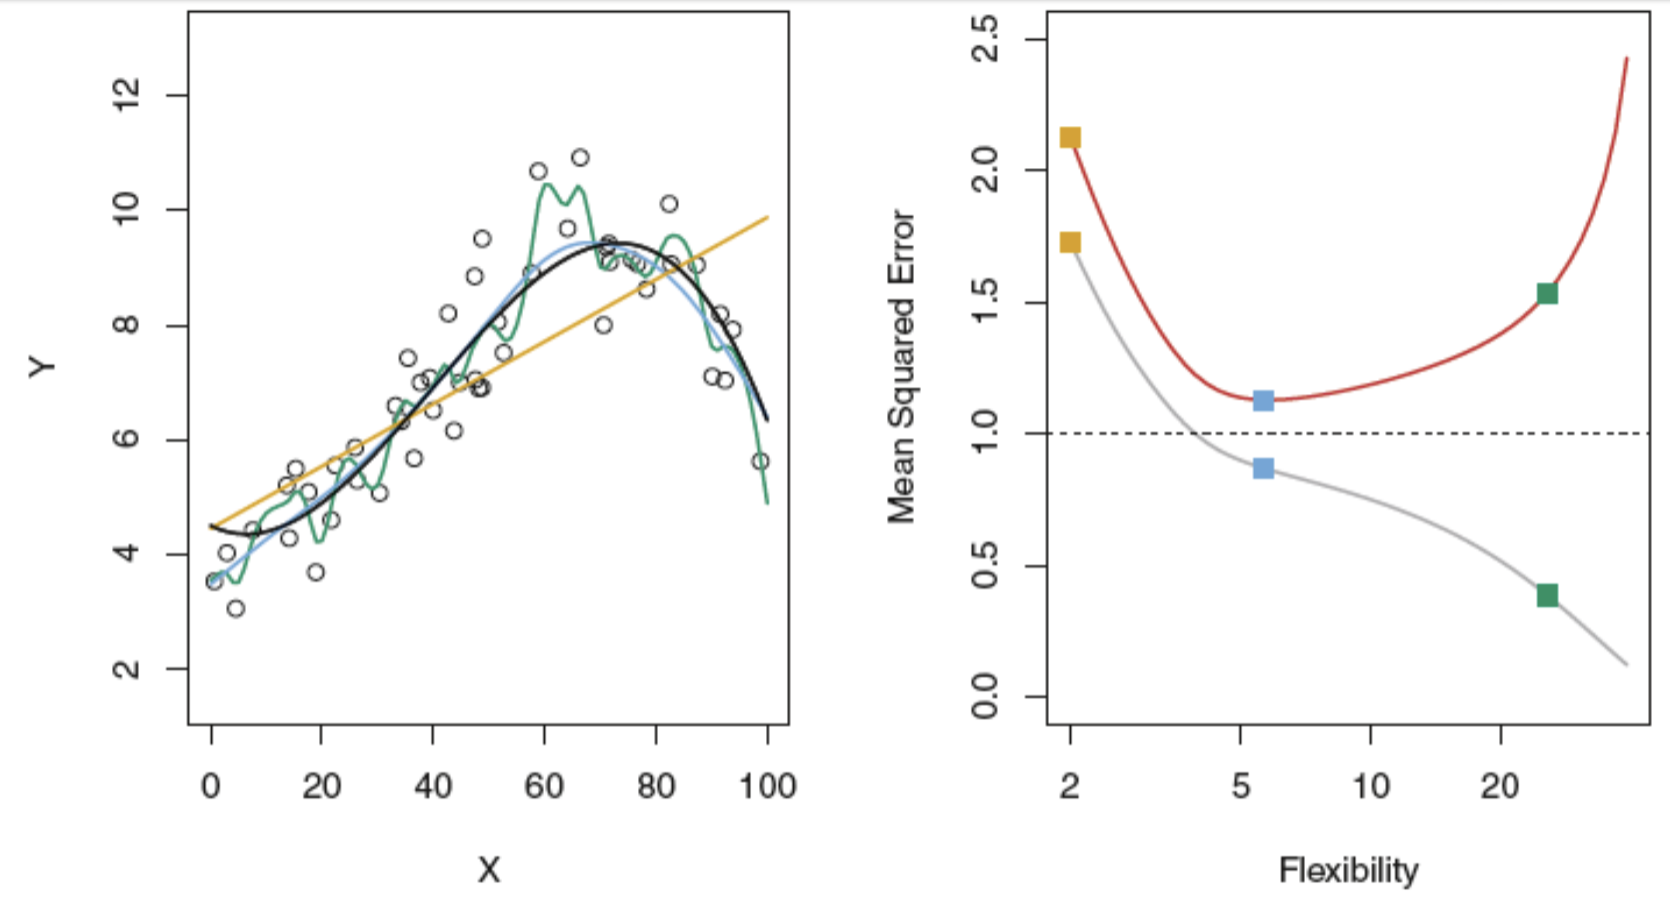
\includegraphics[width=0.7\textwidth]{fotos/21.png}
\caption{Izquierda: se muestran tres estimaciones sobre los datos simulados; una recta de regresión (naranja) y dos splines (azul y verde). Derecha: se muestran las curvas del MSE de \textit{train} (gris) y \textit{test} (rojo). Los cuadrados representan el valor del MSE de cada uno de los tres ajustes de la izquierda.}
\label{fig:4.1}
\end{figure}

\subsection{Compromiso entre \textit{bias} y varianza}

Se puede demostrar que el MSE de \textit{test} esperado, para un valor $x_0$ dado, puede descomponerse en la suma de tres cantidades fundamentales: la varianza de $\hat{f}(x_0)$, el \textit{bias} al cuadrado de $\hat{f}(x_0)$ y la varianza del término de error $\epsilon$. Esto es 
\begin{equation}
\text{MSE} \equiv E(y_0 - \hat{f}(x_0))^2 = \text{Var}(\hat{f}(x_0)) + [\text{Bias}(\hat{f}(x_0))]^2 + \text{Var}(\epsilon)
\label{eq:2.7}
\end{equation}

Aquí, el MSE de \textit{test} esperado es el promedio de numerosas estimaciones de $f$ usando un gran número de conjuntos de entrenamiento, comprobados todos sobre $x_0$. El primer término se refiere a la cantidad en la que cambiaría $\hat{f}$ si se estimara usadno un conjunto diferente de entrenamiento. El término de \textit{bias} hace referencia al error introducido por aproximar el problema real por uno mucho más simple, y el último término se corresponde con el error irreducible (el MSE nunca podrá estar por debajo de este). \\

La ecuación (\ref{eq:2.7}) muestra que, para minimizar el error de \textit{test} esperado, se necesita seleccionar un método de aprendizaje estadístico que consiga baja varianza y bajo \textit{bias}. La varianza es, por definición, no negativa, así como el cuadrado del \textit{bias}. De este modo, el MSE esperado de \textit{test} nunca puede ser menor que $\text{Var}(\epsilon)$. \\

\begin{figure}[h]
\centering
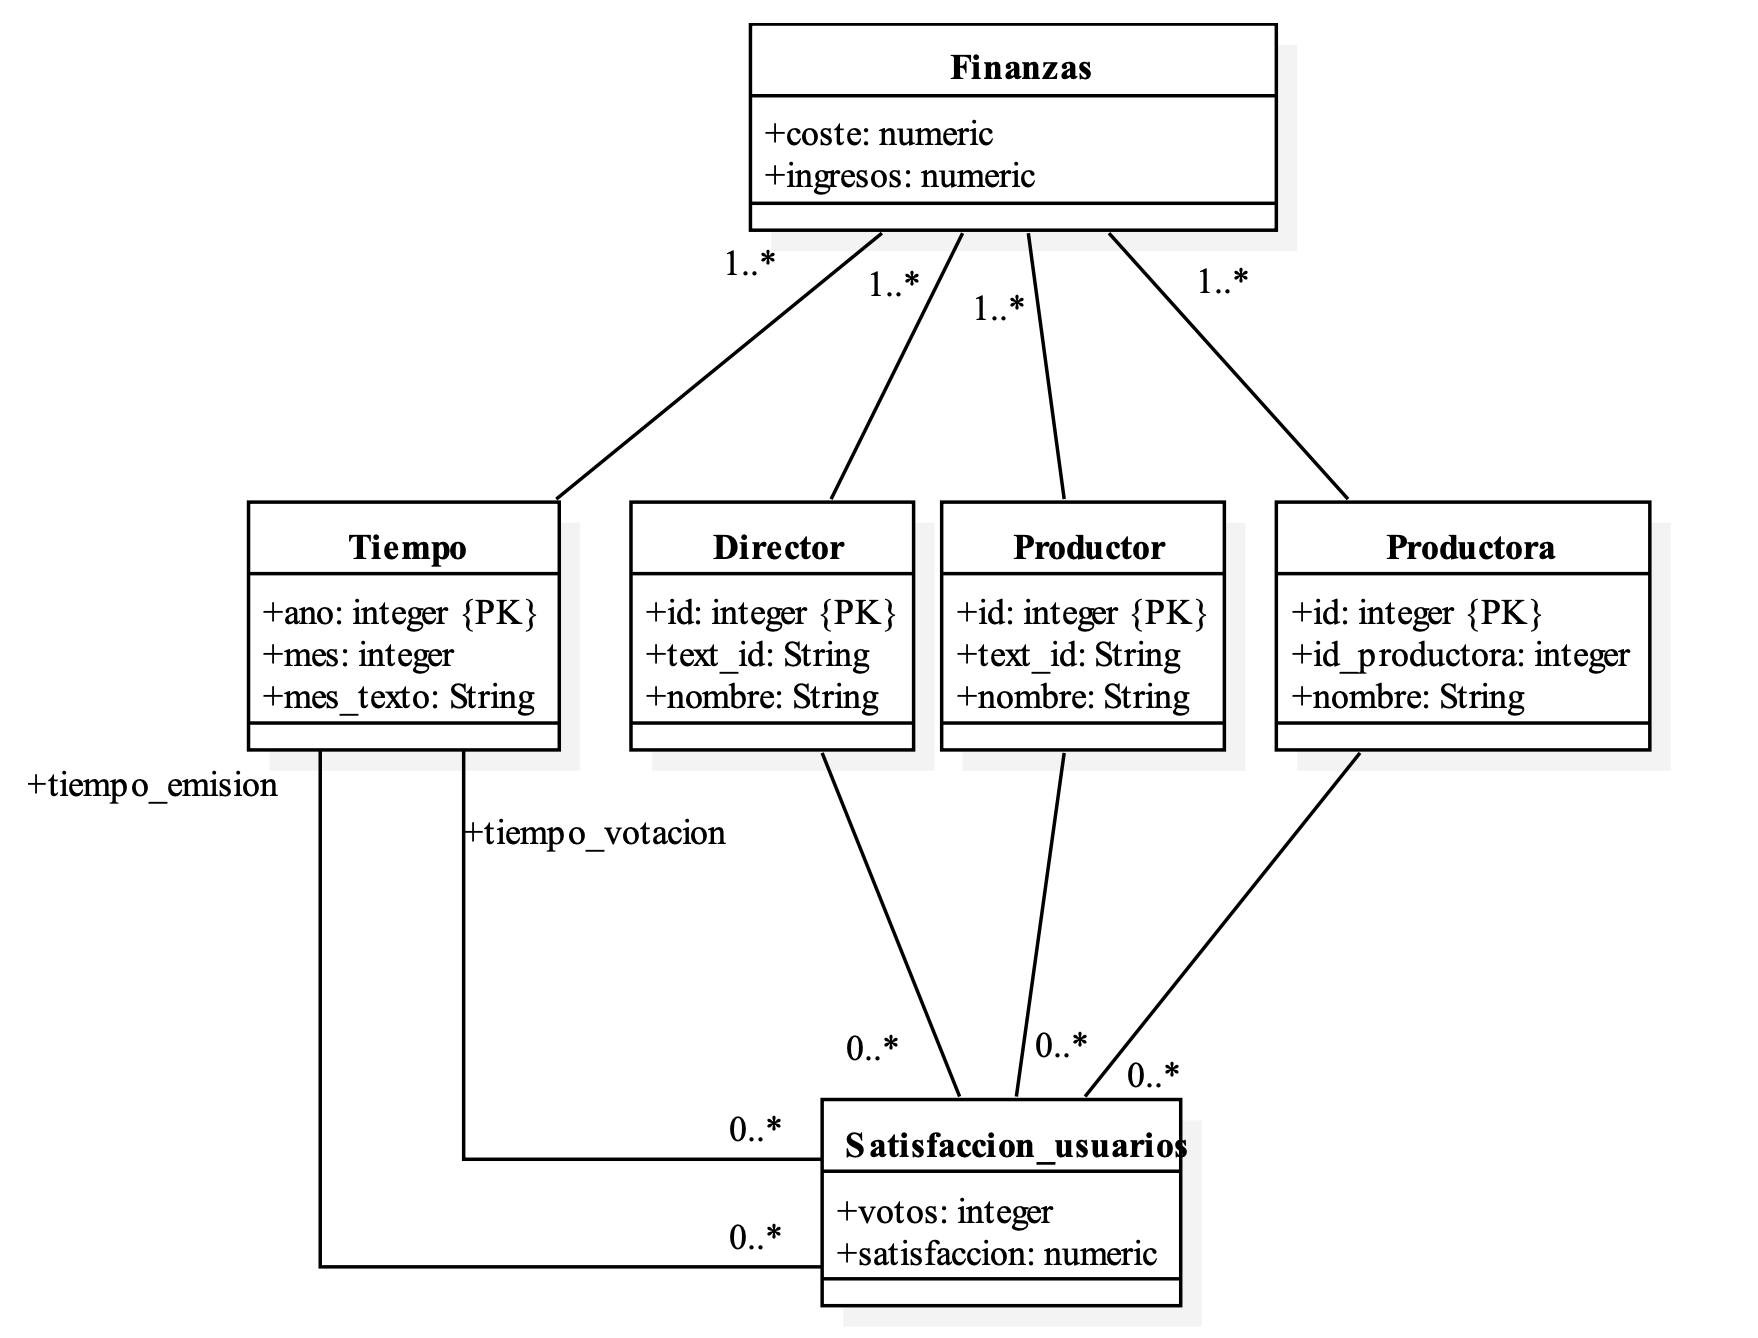
\includegraphics[width=0.8\textwidth]{fotos/3.png}
\caption{\textit{Bias} al cuadrado (azul), varianza (naranja), $\text{Var}(\epsilon)$ (línea discontinua) y MSE de \textit{test} (rojo) para tres conjuntos de datos distintos. Las líneas punteadas verticales indican el nivel de flexibilidad correspondiente al menor MSE de \textit{test}. Al aumentar la flexibilidad, primero el \textit{bias} tiende a disminuir más rápido que la varianza aumenta. Sin embargo, llega un punto en el que aumentar la flexibilidad tiene poco impacto en el \textit{bias}, pero incrementa significativamente la varianza.}
\label{fig:3}
\end{figure}

Generalmente, cuánto más flexible (complejo) sea el método usado, mayor será la varianza y menor el \textit{bias}. Así, el cambio relativo entre ambas determina si el MSE de \textit{test} aumenta o disminuye. Esta relación se puede ver en la figura \ref{fig:3}. A igualdad de resultados, se elegirán modelos sencillos, ya que tiene mayor capacidad de generalizacion. 

\section{Contexto de clasificación}

El entorno de clasificación general, así como el clasificador de Bayes, se describen con detalle en la sección \ref{sec:3.1}. Además, se definen otras herramientas para evaluar el rendimiento de un clasificador:
\begin{itemize}
\item Matriz de confusión (tabla \ref{tb:4.6}). En la tabla \ref{tb:4.7} se enumera muchas de las medidas de rendimiento populares que se utilizan en este contexto. 
\begin{table}[h]
\centering
\begin{tabular}{c|c|c|c}
\hline
Clase verdadera & \multicolumn{3}{c}{Clase predicha} \\ \hline
& $-$ o nulo & $+$ or no nulo & Total \\ \hline
$-$ o nulo & True Neg. (TN) & False Pos. (FP) & N \\ \hline
$+$ o no nulo & False Neg. (FN) & True Pos. (TP) & P \\ \hline
Total & N* & P* &  \\ \hline
\end{tabular}
\caption{Matriz de confusión. Posibles resultados al aplicar un clasificador a una población.}
\label{tb:4.6}
\end{table}
\begin{table}[h]
\centering
\resizebox{\textwidth}{!}{
\begin{tabular}{c|c}
\hline \hline
Nombre & Definición \\ \hline \hline
Precisión & $\text{TP}/\text{P}^* = \text{TP}/(\text{TP} + \text{FP})$ \\ 
Recall, sensitividad, \textit{true positive rate} (TPR) & $\text{TP}/\text{P} = \text{TP}/(\text{TP} + \text{FN})$ \\ 
Especificidad, \textit{true negative rate} (TNR) & $\text{TN}/\text{N} = \text{TN}/(\text{TN} + \text{FP})$ \\ 
Tasa de falsos positivos (FPR) & $\text{FP}/\text{N} = \text{FP}/(\text{TN} + \text{FP})$ \\ 
Tasa de falsos negativos (FNR) & $\text{FN}/\text{P} = \text{FN}/(\text{TP} + \text{FN})$ \\ 
\textit{Accuracy} & $(\text{TP} + \text{TN})/(\text{P} + \text{N}) = (\text{TP} + \text{TN})/(\text{TP} + \text{TN} + \text{FP} + \text{FN})$ \\ \hline
\end{tabular}
}
\caption{Medidas de rendimiento para clasificación.}
\label{tb:4.7}
\end{table}
\item La curva ROC es un gráfico popular para mostrar simultáneamente los dos tipos de errores para todos los umbrales posibles. El rendimiento general de un clasificador, resumido en todos los umbrales posibles, se da por el área bajo la curva (AUC). Una curva ROC ideal abrazará la esquina superior izquierda, por lo que cuanto mayor sea el AUC, mejor será el clasificador. Se espera que un clasificador que no funcione mejor que el azar tenga un AUC de 0.5 (cuando se evalúa en un conjunto de prueba independiente no utilizado en el entrenamiento del modelo). Las curvas ROC son útiles para comparar diferentes clasificadores, ya que tienen en cuenta todos los umbrales posibles.
\begin{figure}[h]
\centering
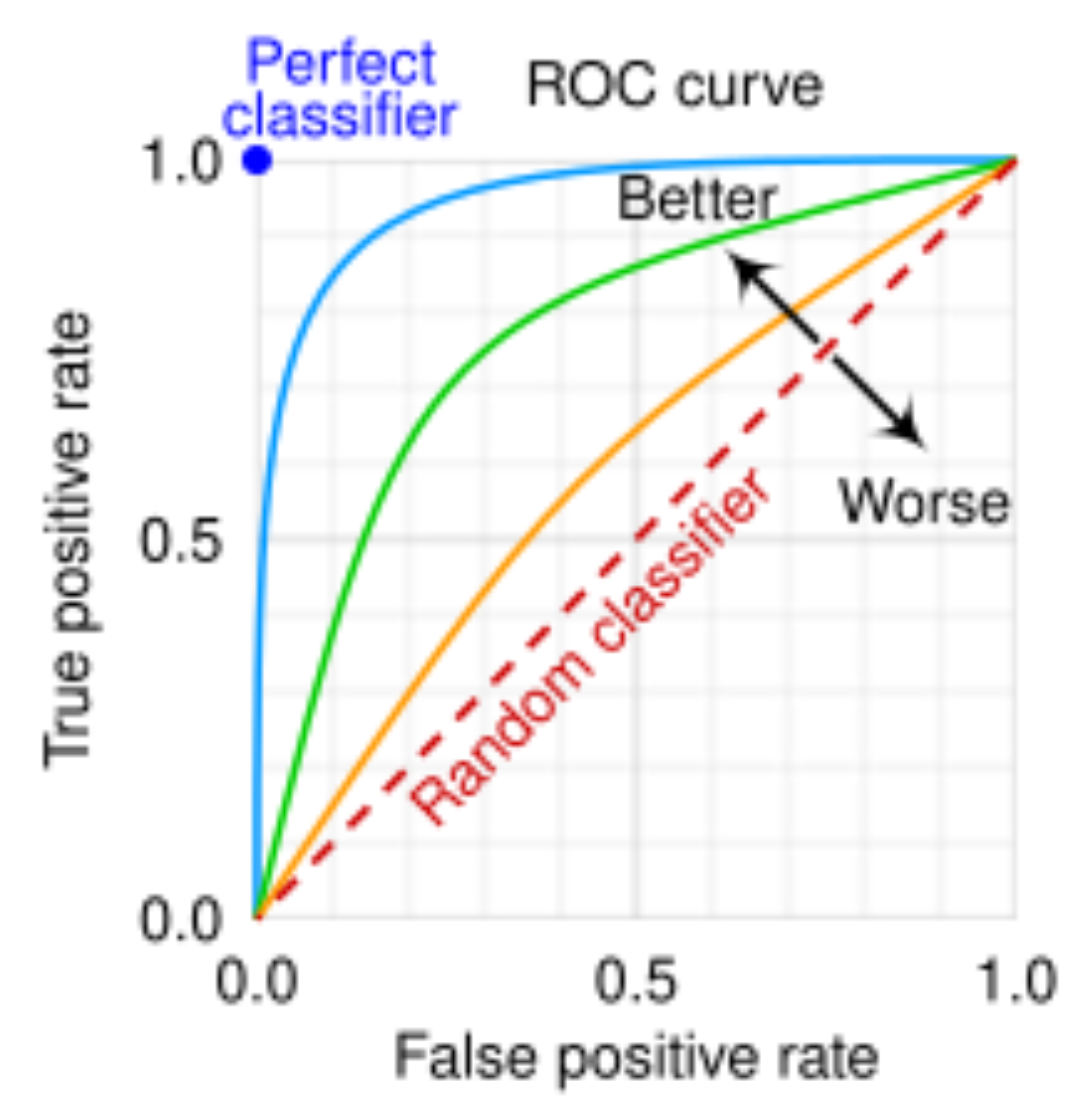
\includegraphics[width=0.4\textwidth]{fotos/22.png}
\caption{Curva ROC para un clasificador.}
\end{figure}
\end{itemize}

\section{Métodos de remuestreo}

En una situación ideal, con el datos suficientes, se podría dividir el conjunto de datos en dos partes: una para entrenar el modelo y otra para evaluarlo. A su vez, se podría dividir el conjunto de datos de entrenamiento en dos partes: una para ajustar el modelo y otra para seleccionar el mejor (validación), estimando sobre él el MSE. Sin embargo, en la práctica, esto no es posible. \\

Los métodos de remuestreo son una herramienta indispensable en la estadística moderna. Implican extraer repetidamente muestras de un conjunto de entrenamiento y volver a ajustar un modelo de interés en cada muestra para obtener información adicional sobre el modelo ajustado. Este enfoque puede permitirnos obtener información que no estaría disponible al ajustar el modelo solo una vez utilizando la muestra de entrenamiento original. Hay principalmente dos tipos: validación cruzada y \textit{bootstrap}, aquí solo trataremos la validación cruzada.

\subsection{Validación cruzada}

En ausencia de un conjunto de prueba designado muy grande que pueda usarse para estimar directamente la tasa de error de prueba, se pueden usar una serie de técnicas para estimar esta cantidad utilizando los datos de entrenamiento disponibles. Aquí consideramos una clase de métodos que estiman la tasa de error de prueba reteniendo un subconjunto de las observaciones de entrenamiento del proceso de ajuste, y luego aplicando el método de aprendizaje estadístico a esas observaciones retenidas. Los métodos de validación cruzada son de aplicación general y pueden usarse con cualquier método de aprendizaje estadístico. \\

En las subsecciones siguientes, a no ser que se especifique lo contrario, asumimos un problema de regresión con una respuesta cuantitativa. Sin embargo, los conceptos clave permanecen iguales sin importar si la respuesta es cuantitativa o cualitativa.

\subsubsection{Enfoque del Conjunto de Validación}

Supongamos que nos gustaría estimar el error de prueba asociado con el ajuste de un método de aprendizaje estadístico particular en un conjunto de observaciones. El enfoque del conjunto de validación, mostrado en la figura \ref{fig5.1}, es una estrategia muy simple para esta tarea. Implica dividir aleatoriamente el conjunto disponible de observaciones en dos partes, un conjunto de entrenamiento y un conjunto de validación o conjunto de retención. El modelo se ajusta en el conjunto de entrenamiento, y el modelo ajustado se utiliza para predecir las respuestas para las observaciones en el conjunto de validación. La tasa de error del conjunto de validación resultante, típicamente evaluada usando el MSE en el caso de una respuesta cuantitativa, proporciona una estimación de la tasa de error de prueba. \\

\begin{figure}[h]
\centering
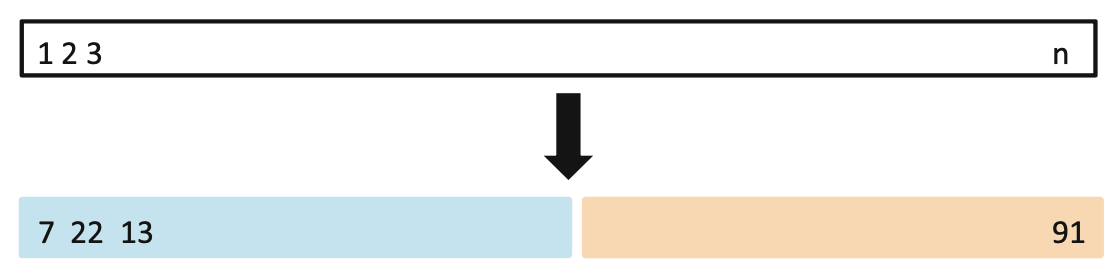
\includegraphics[width=0.7\textwidth]{fotos/23.png}
\caption{División de un conjunto de datos en un conjunto de entrenamiento y un conjunto de validación.}
\label{fig5.1}
\end{figure}

\begin{figure}[h]
\centering
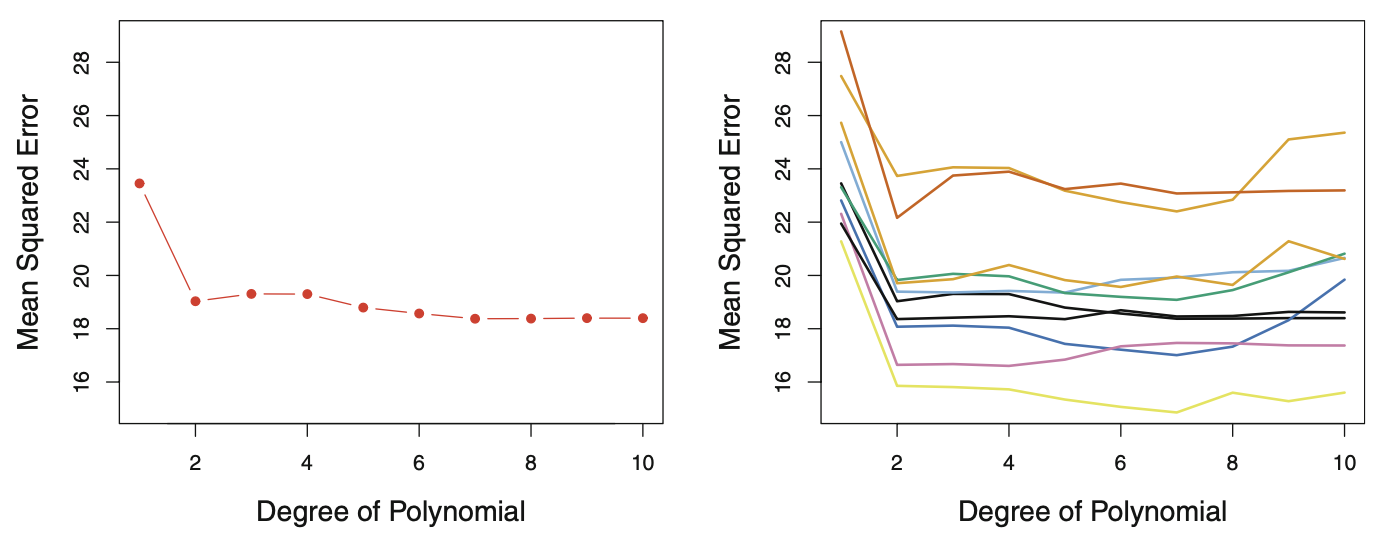
\includegraphics[width=0.8\textwidth]{fotos/24.png}
\caption{Ejemplo del enfoque del conjunto de validación para predecir una variable en función de funciones polinómicas de un predictor (en general, se pueden hacer las combinaciones de predictores que queramos. Por ejemplo, en clasificación, si se tienen dos predictores, es común probar con sus combinaciones $X_1^2$, $X_2^2$, $X_1X_2 \dots$). A la izquierda se tiene la estimación del MSE con una única división de entrenamiento y validación. A la derecha, se tiene la estimación del MSE con 10 divisiones aleatorias de las observaciones. Esto ilustra la variabilidad en la estimación del MSE de \textit{test}.}
\label{fig5.2}
\end{figure}

El enfoque del conjunto de validación es conceptualmente simple y fácil de implementar. Pero tiene dos posibles inconvenientes:

\begin{itemize}
\item La estimación de la tasa de error de prueba mediante validación puede ser altamente variable, dependiendo precisamente de qué observaciones se incluyan en el conjunto de entrenamiento y cuáles se incluyan en el conjunto de validación.
\item En el enfoque de validación, solo un subconjunto de las observaciones que se incluyen en el conjunto de entrenamiento en lugar de en el conjunto de validación se utiliza para ajustar el modelo. Dado que los métodos estadísticos tienden a desempeñarse peor cuando se entrenan con menos observaciones, esto sugiere que la tasa de error del conjunto de validación puede tender a sobreestimar la tasa de error de prueba para el modelo ajustado con todo el conjunto de datos.
\end{itemize}

\subsection{Validación cruzada \textit{Leave-One-Out}}

La validación cruzada leave-one-out (LOOCV) está estrechamente relacionada con el enfoque del conjunto de validación, pero intenta abordar las desventajas de dicho método. \\

\begin{figure}[h]
\centering
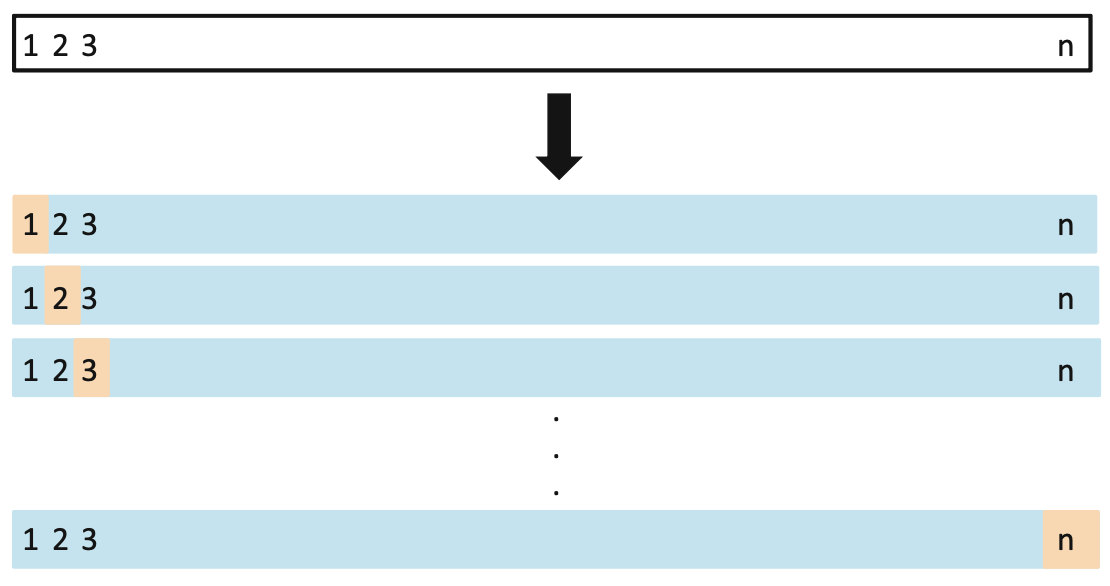
\includegraphics[width=0.7\textwidth]{fotos/25.png}
\caption{Ilustración de LOOCV.}
\label{fig5.3}
\end{figure}

Al igual que el enfoque del conjunto de validación, LOOCV implica dividir el conjunto de observaciones en dos partes. Sin embargo, en lugar de crear dos subconjuntos de tamaño comparable, se utiliza una sola observación $(x_1, y_1)$ para el conjunto de validación, y las observaciones restantes $\{(x_2, y_2), \dots, (x_n, y_n)\}$ conforman el conjunto de entrenamiento. El método de aprendizaje estadístico se ajusta con las $n-1$ observaciones de entrenamiento, y se realiza una predicción $\hat{y}_1$ para la observación excluida, utilizando su valor $x_1$. Dado que $(x_1, y_1)$ no se utilizó en el proceso de ajuste, $MSE_1 = (y_1 - \hat{y}_1)^2$ proporciona una estimación aproximadamente no sesgada del error de prueba. Sin embargo, aunque $MSE_1$ es no sesgado para el error de prueba, es una estimación pobre porque es altamente variable, ya que se basa en una sola observación $(x_1, y_1)$. \\

Se puede repetir el procedimiento seleccionando $(x_2, y_2)$ para los datos de validación, entrenando el procedimiento de aprendizaje estadístico con las $n-1$ observaciones $\{(x_1, y_1), (x_3, y_3),$  $\dots, (x_n, y_n)\}$ y calculando $MSE_2 = (y_2 - \hat{y}_2)^2$. Repetir este enfoque $n$ veces produce $n$ errores al cuadrado, $MSE_1, \dots, MSE_n$. La estimación LOOCV para el MSE de prueba es el promedio de estas $n$ estimaciones del error de prueba:
\begin{equation}
\text{CV}_{(n)} = \frac{1}{n} \sum_{i=1}^{n} \text{MSE}_i 
\end{equation}

LOOCV tiene ventajas sobre el enfoque del conjunto de validación. Primero, tiene mucho menos \textit{bias}. En LOOCV, se ajusta repetidamente el método de aprendizaje estadístico utilizando conjuntos de entrenamiento que contienen $n-1$ observaciones, casi tantas como las que están en el conjunto de datos completo. Esto contrasta con el enfoque del conjunto de validación, en el cual el conjunto de entrenamiento típicamente es alrededor de la mitad del tamaño del conjunto de datos original. En consecuencia, el enfoque LOOCV tiende a sobrestimar la tasa de error de prueba mucho menos que el enfoque del conjunto de validación. Segundo, en contraste con el enfoque de validación, que dará resultados diferentes cuando se aplique repetidamente debido a la aleatoriedad en las divisiones del conjunto de entrenamiento/validación, realizar LOOCV múltiples veces siempre dará los mismos resultados: no hay aleatoriedad en las divisiones del conjunto de entrenamiento/validación. \\

\begin{figure}[h]
\centering
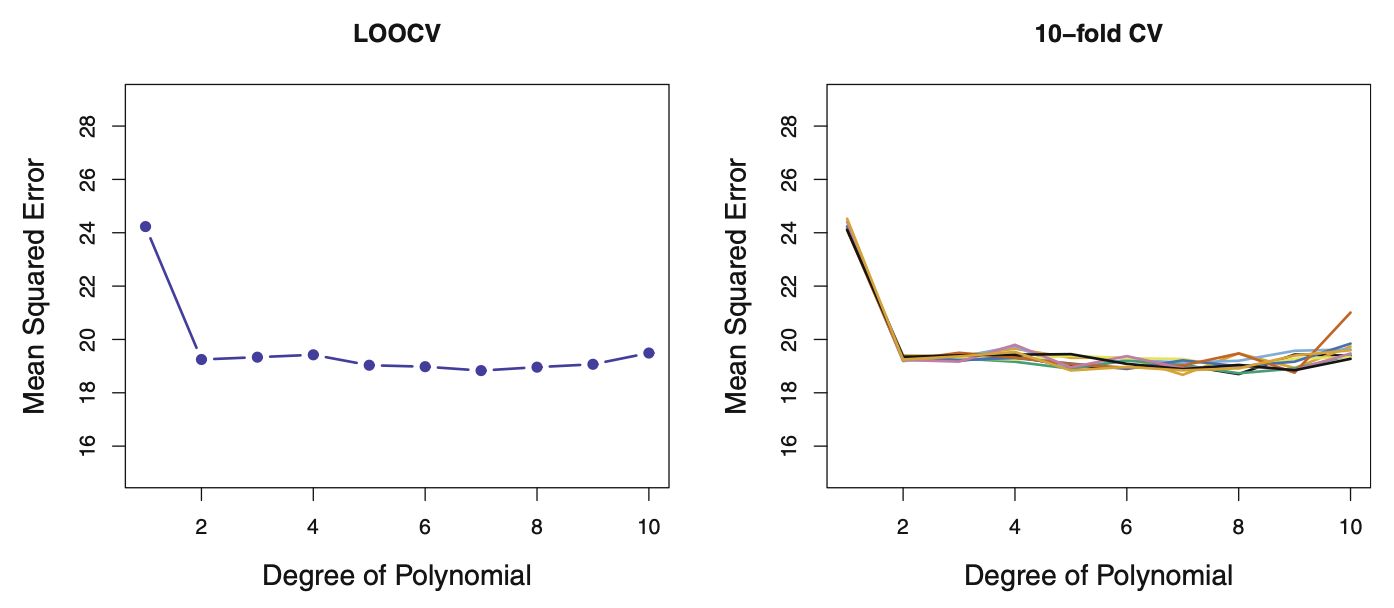
\includegraphics[width=0.8\textwidth]{fotos/26.png}
\caption{LOOCV sobre el mismo conjunto de datos de la figura \ref{fig5.2}.}
\label{fig5.4}
\end{figure}

LOOCV puede ser costoso de implementar, ya que el modelo debe ajustarse $n$ veces. Esto puede consumir mucho tiempo si $n$ es grande y si cada modelo individual es lento de ajustar. Para regresión lineal por mínimos cuadrados o polinómica, existe una forma de que el costo de LOOCV sea el mismo que el de un solo ajuste del modelo. Por la siguiente fórmula:
\begin{equation}
\text{CV}_{(n)} = \frac{1}{n} \sum_{i=1}^{n} \left(\frac{y_i - \hat{y}_i}{1 - h_i}\right)^2
\label{eq:5.2}
\end{equation}

\noindent donde $\hat{y}_i$ es el $i$-ésimo valor ajustado del ajuste original de mínimos cuadrados, y $h_i$ es la influencia definida por
\begin{equation}
h_i = \frac{1}{n} + \frac{(x_i - \bar{x})^2}{\sum_{i'=1}^n (x_{i'} - \bar{x})^2}
\end{equation}

Esto es similar al MSE ordinario, excepto que el residuo $i$-ésimo se divide por $1 - h_i$. La influencia se encuentra entre $1/n$ y $1$, y refleja la cantidad que una observación influye en su propio ajuste. Por lo tanto, los residuos para puntos de alta influencia se inflan en esta fórmula por exactamente la cantidad correcta para que esta igualdad se cumpla. \\

LOOCV es un método muy general y puede usarse con cualquier tipo de modelado predictivo. La fórmula (\ref{eq:5.2}) no se cumple en general, en cuyo caso el modelo debe ajustarse $n$ veces.

\begin{figure}[h]
\centering
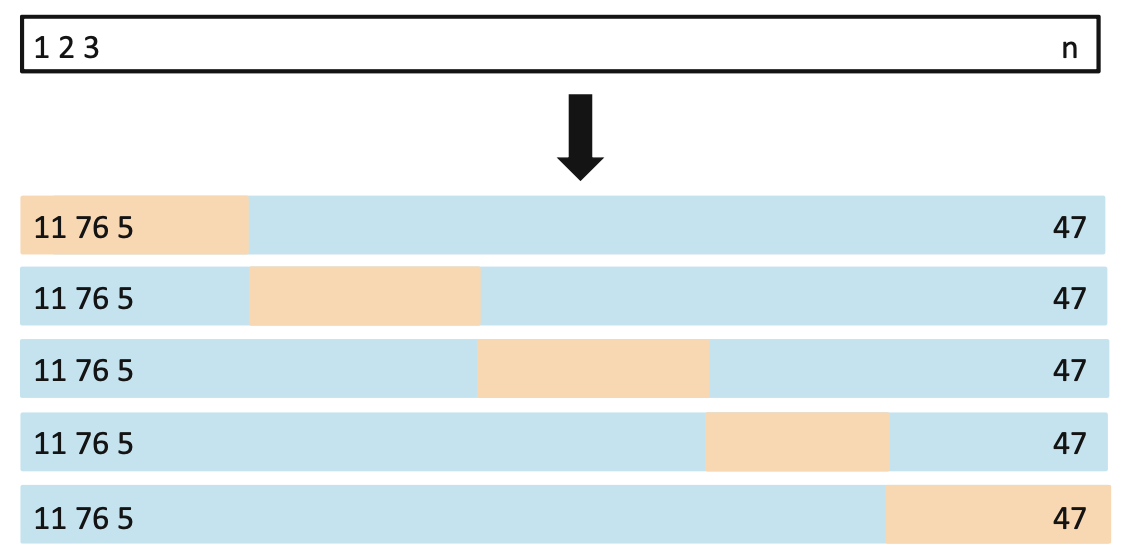
\includegraphics[width=0.8\textwidth]{fotos/27.png}
\caption{Validación cruzada k-fold, con $k = 5$.}
\label{fig:5.5}
\end{figure}

\subsection{Validación Cruzada k-Fold}

Una alternativa a LOOCV es la validación cruzada k-fold. Este enfoque implica dividir aleatoriamente el conjunto de observaciones en $k$ grupos, de tamaño aproximadamente igual. El primer grupo se trata como un conjunto de validación, y el método se ajusta con los $k-1$ grupos restantes. Luego, se calcula el error cuadrático medio, $MSE_1$, en las observaciones del grupo retenido. Este procedimiento se repite $k$ veces; cada vez, un grupo diferente de observaciones se trata como un conjunto de validación. Este proceso resulta en $k$ estimaciones del error de prueba, $MSE_1, MSE_2, \dots, MSE_k$. La estimación de CV \textit{k-fold} se calcula promediando estos valores,
\begin{equation}
\text{CV}_{(k)} = \frac{1}{k} \sum_{i=1}^{k} \text{MSE}_i
\end{equation}

La figura \ref{fig:5.5} ilustra el enfoque de CV \textit{k-fold}. LOOCV es por tanto un caso especial de \textit{k-fold} CV en el que $k$ se establece igual a $n$. En la práctica, típicamente se realiza CV k-fold usando $k = 5$ o $k = 10$. \\

Cuando examinamos datos reales, no conocemos el verdadero MSE de prueba, por lo que es difícil determinar la precisión de la estimación de la validación cruzada. Sin embargo, si examinamos datos simulados, entonces podemos calcular el verdadero MSE de prueba y, por lo tanto, evaluar la precisión de nuestros resultados de validación cruzada. 

\begin{figure}[h]
\centering
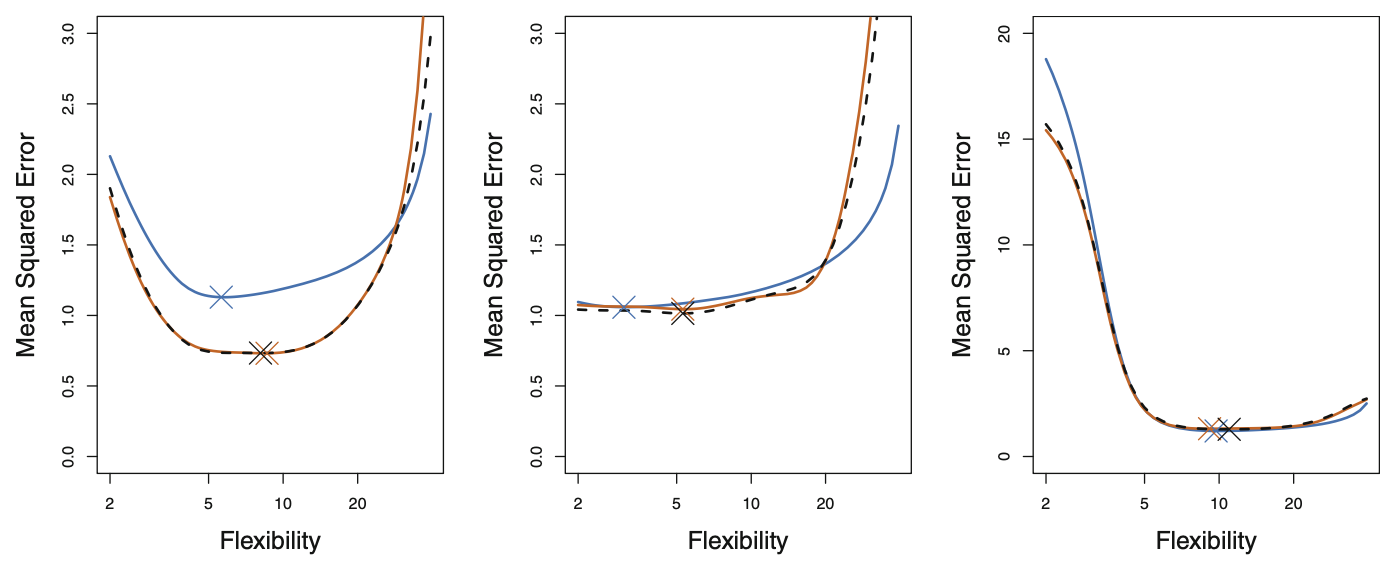
\includegraphics[width=0.8\textwidth]{fotos/28.png}
\caption{Estimaciones de validación cruzada y las tasas de error de prueba reales que resultan de aplicar splines de suavizado a conjuntos de datos simulados. El verdadero MSE de prueba se muestra en azul. Las líneas discontínuas negras y sólidas naranjas muestran respectivamente las estimaciones de LOOCV y CV de 10 grupos. En los tres gráficos, las dos estimaciones de validación cruzada son muy similares. En el panel derecho, el verdadero MSE de prueba y las curvas de validación cruzada son casi idénticos. En el panel central, los dos conjuntos de curvas son similares en los grados inferiores de flexibilidad, mientras que las curvas de CV sobreestiman el MSE del conjunto de prueba para grados superiores de flexibilidad. En el panel izquierdo, las curvas de CV tienen la forma general correcta, pero subestiman el verdadero MSE de prueba.}
\label{fig5.6}
\end{figure}

\subsection{Compromiso \textit{bias}-varianza para la validación cruzada k-Fold}

Una ventaja menos obvia pero más importante de la CV \textit{k-fold} es que a menudo proporciona estimaciones más precisas de la tasa de error de prueba que LOOCV. Esto tiene que ver con una compensación \textit{bias}-varianza. \\

El enfoque del conjunto de validación puede llevar a sobreestimar la tasa de error de prueba, ya que en este enfoque el conjunto de entrenamiento utilizado para ajustar el método de aprendizaje estadístico contiene solo la mitad de las observaciones del conjunto de datos completo. Usando esta lógica, no es difícil ver que LOOCV dará estimaciones aproximadamente no sesgadas del error de prueba, ya que cada conjunto de entrenamiento contiene $n-1$ observaciones, que es casi tantas como el número de observaciones en el conjunto de datos completo. Y realizar CV k-fold para, por ejemplo, $k = 5$ o $k = 10$ llevará a un nivel intermedio de sesgo, ya que cada conjunto de entrenamiento contiene $(k-1)n/k$ observaciones, menos que en el enfoque LOOCV, pero sustancialmente más que en el enfoque del conjunto de validación. Por lo tanto, desde la perspectiva de la reducción del \textit{bias}, está claro que LOOCV es preferible a la CV k-fold. \\

Sin embargo, sabemos que el \textit{bias} no es la única fuente de preocupación en un procedimiento de estimación; también debemos considerar la varianza del procedimiento. Resulta que LOOCV tiene una varianza más alta que la CV k-fold con $k < n$. Cuando realizamos LOOCV, estamos promediando los resultados de $n$ modelos ajustados, cada uno de los cuales se entrena con un conjunto de observaciones casi idéntico; por lo tanto, estos resultados están altamente correlacionados positivamente entre sí. En contraste, cuando realizamos CV k-fold con $k < n$, estamos promediando los resultados de $k$ modelos ajustados que están algo menos correlacionados entre sí, ya que la superposición entre los conjuntos de entrenamiento en cada modelo es menor. Dado que la media de muchas cantidades altamente correlacionadas tiene una varianza mayor que la media de muchas cantidades que no están tan altamente correlacionadas, la estimación del error de prueba resultante de LOOCV tiende a tener una varianza más alta que la estimación del error de prueba resultante de la CV \textit{k-fold}. \\

Para resumir, existe una compensación sesgo-varianza asociada con la elección de $k$ en la validación cruzada k-fold. Típicamente, dadas estas consideraciones, se realiza validación cruzada k-fold usando $k = 5$ o $k = 10$, ya que se ha demostrado empíricamente que estos valores producen estimaciones de la tasa de error de prueba que no sufren ni de un \textit{bias} excesivamente alto ni de una varianza muy alta.

\subsection{Validación Cruzada en Problemas de Clasificación}

La validación cruzada también puede ser un enfoque muy útil en el entorno de clasificación cuando $Y$ es cualitativa. En este entorno, la validación cruzada funciona tal como se describió anteriormente en este capítulo, excepto que en lugar de usar el MSE para cuantificar el error de prueba, utilizamos el número de observaciones mal clasificadas. Por ejemplo, en el entorno de clasificación, la tasa de error de LOOCV toma la forma
\begin{equation}
\text{CV}_{(n)} = \frac{1}{n} \sum_{i=1}^{n} \text{Err}_i
\end{equation}

\noindent donde $\text{Err}_i = I(y_i \neq \hat{y}_i)$. La tasa de error de CV \textit{k-fold} y las tasas de error del conjunto de validación se definen de manera análoga. \\

\begin{figure}[h]
\centering
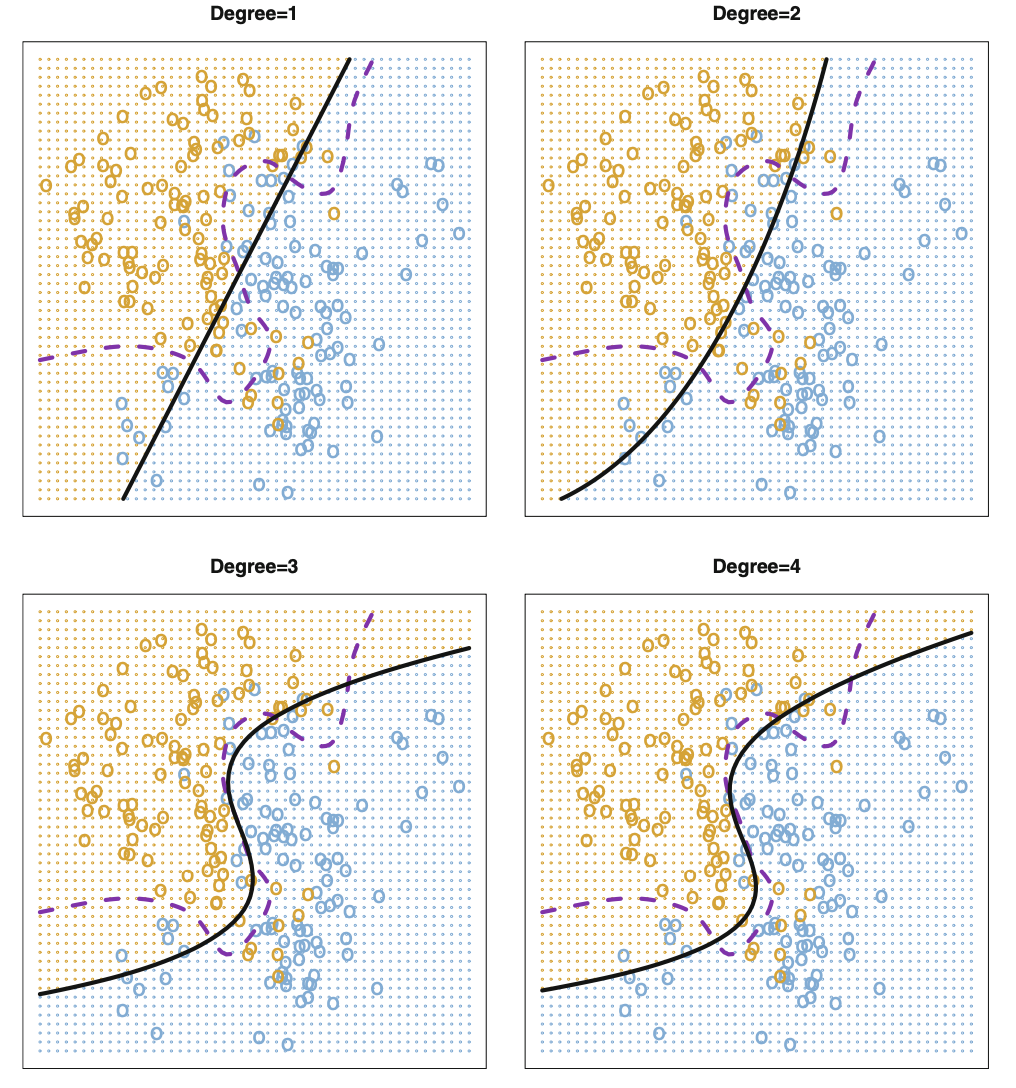
\includegraphics[width=0.8\textwidth]{fotos/29.png}
\caption{Ajustes de regresión logística en una clasificación bidimensional. La frontera de decisión de Bayes se representa por una línea discontinua morada. Las frontera de decisiones estimadas por regresión logística lineal, cuadrática, cúbica y cuártica se muestran en negro.}
\label{fig:5.7}
\end{figure}

\begin{figure}[h]
\centering
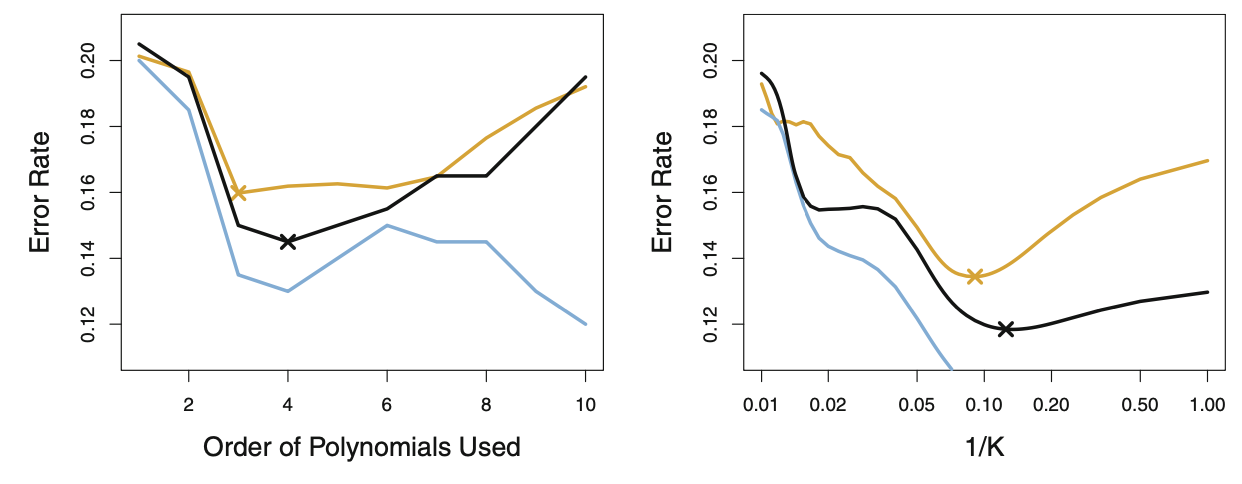
\includegraphics[width=0.8\textwidth]{fotos/30.png}
\caption{Error de \textit{test} (marrón), error de entrenamiento (azul) y error de CV con 10 grupos (negro) en datos bidimensionales. A la izquierda una regresión logística usando funciones polinómicas de los predictores. A la derecha el clasificador KNN con diferentes valores de $K$.}
\label{fig:5.8}
\end{figure}

En la práctica, para datos reales, la frontera de decisión de Bayes y las tasas de error de prueba son desconocidas. Para decir entre modelos, podemos usar la validación cruzada para tomar esta decisión. Esto lo vemos en la figura \ref{fig:5.8} . Como hemos visto anteriormente, la tasa de error de entrenamiento tiende a disminuir a medida que aumenta la flexibilidad del ajuste (aunque la tasa de error de entrenamiento no disminuye de manera monótona, tiende a disminuir en general a medida que aumenta la complejidad del modelo). En contraste, el error de prueba muestra una característica en forma de U. La tasa de error de CV de 10 grupos proporciona una buena aproximación a la tasa de error de prueba. Aunque subestima un poco la tasa de error, alcanza un mínimo cuando se usan polinomios de cuarto orden, lo cual está muy cerca del mínimo de la curva de prueba, que ocurre cuando se usan polinomios de tercer orden. De hecho, utilizar polinomios de cuarto orden probablemente llevaría a un buen rendimiento en el conjunto de prueba, ya que la verdadera tasa de error de prueba es aproximadamente la misma para polinomios de tercer, cuarto, quinto y sexto orden. 

\begin{example}
Mínimos cuadrados es un modelo sobreajustado. En regresión Ridge y Lasso, el hiperparámetro es $\lambda$, y la flexibilidad va con $1/\lambda$, a mayor $\lambda$ el modelo tiende al sobreajuste. 
\end{example}

\subsubsection{Regla de una desviación estándar}

Se calcula la desviación estándar de los errores de validación cruzada para cada modelo. Se selecciona el modelo más simple cuyo error de validación cruzada está dentro de una desviación estándar del modelo con el menor error de validación cruzada.

\subsubsection{Forma correcta de hacer validación cruzada}

\begin{itemize}
\item Si no se hace selección de modelos:
\begin{itemize}
\item Dividir la muestra en $k$ grupos. Para cada uno:
\begin{itemize}
\item Entrenar al modelo con todos los grupos menos el $k$-ésimo.
\item Probar el modelo con el grupo $k$-ésimo.
\end{itemize}
\item Calcular la media y desviación estándar del error de \textit{test} estimado.
\end{itemize}
\item Si se hace selección de modelos: se deben estimar los hiperparámos (sobre el conjunto de validación)
\begin{itemize}
\item Dividir la muestra en grupos de entrenamiento y validación.
\item Dividir el grupo de entrenamiento en $k$ grupos. Para cada combinación de hiperparámetros:
\begin{itemize}
\item Para cada grupo:
\begin{itemize}
\item Entrenar al modelo con todos los grupos menos el $k$-ésimo.
\item Probar el modelo con el grupo $k$-ésimo.
\end{itemize}
\item Calcular la media y desviación estándar del error de validación cruzada.
\end{itemize}
\item Seleccionar los hiperparámetros con la regla de una desviación estándar.
\item Entrenar el modelo con los hiperparámetros seleccionados y todos los datos de entrenamiento (añadir más datos sin sesgo no genera sobreentrenamiento).
\item Probar el modelo con el conjunto de \textit{test}.
\end{itemize}
\end{itemize}







\section{Selección de subconjuntos} \label{sec:4.1}

\subsection{Selección del mejor subconjunto}

Para hacer la selección del mejor subconjunto, se debe ajustar una regresión de mínimos cuadrados distinta para cada combinación de los $p$ predictores. Esto es, se ajustan todos los $p$ modelos que contienen exactamente un predictor, los $\binom{p}{2} = p(p-1)/2$ modelos que contienen exactamente dos predictores, y así sucesivamente. Luego, se selecciona el mejor modelo. \\

El problema viene en elegir el mejor de entre las $2^p$ posibilidades consideradas. Esto se suele hacer en dos etapas:
\begin{enumerate}
\item Sea $\mathcal{M}_0$ el modelo nulo que no contiene ningún predictor. Este modelo predice la media de la muestra para cada observación.
\item Para $k = 1, 2, \ldots, p$:
\begin{enumerate}
\item Ajustar todos los $\binom{p}{k}$ modelos que contienen exactamente $k$ predictores.
\item Elegir el mejor modelo entre los $\binom{p}{k}$ modelos, y llamarlo $\mathcal{M}_k$. Aquí, ``mejor'' se refiere a tener el menor RSS o, equivalentemente, el mayor $R^2$. Tras esto, el problema se reduce de $2^p$ posibilidades a $p+1$. 
\end{enumerate}
\item Elegir un único ``mejor'' modelo de entre $\mathcal{M}_0, \dots, \mathcal{M}_p$ usando predicción de error validada de forma cruzada, $C_p$ (AIC), BIC, o $R^2$ ajustado.
\end{enumerate}

Para elegir el mejor modelo hay que elegir entre los $p+1$ modelos $\mathcal{M}_i$, con $i = 0, \dots, p$. Hay que tener en cuenta que el RSS de estos modelos decrece de forma monótona, mientras que el $R^2$ aumenta de forma monótona. Por tanto, si se usa estos estadísticos para elegir el mejor modelo, siempre se acabará con un modelo que incluya todas las variables. El problema es que un RSS bajo o un $R^2$ alto indica un modelo con un error de entrenamiento bajo, mientras que lo que se quiere es elegir un modelo con un error de \textit{test} bajo. Por tanto, en el paso 3, se usa la predicción de error validada de forma cruzada, $C_p$, BIC o $R^2$ ajustado para elegir entre $\mathcal{M}_0, \mathcal{M}_1, \dots, \mathcal{M}_p$. 

\subsection{Selección por pasos}

Por motivos computacionales, la selección del mejor subconjunto no sirve para $p$ grandes, caso donde puede sufrir de porblemas estadísticos. Cuando mayor sea el espacio de búsqueda, mayor será la posibilidad de encontrar modelos que ajusten bien el conjunto de entrenamiento, aunque no tenga buen poder predictivo. Entonces, un gran espacio de búsqueda puede conducir a \textit{overfitting} y una gran variación de los coeficientes estimados. Los modelos de selección por pasos exploran un conjunto restringido de modelos, por lo que resultan una buena alterantiva. 

\subsubsection{Selección por pasos hacia adelante}

Este método resulta más eficiente computacionalmente que la selcción del mejor subconjunto. Este método comienza con un modelo que no contenga predictores, y va añadiendo predictores al modelo, uno a uno, hasta que todos los predictores están dentro del modelo. En particular, en cada paso, se añade la variable que dé la mayor mejora al ajuste. Formalmente:
\begin{enumerate}
\item Sea $\mathcal{M}_0$ el modelo nulo, que no contiene predictores.
\item Para $k = 0, \dots, p-1$:
\begin{enumerate}
\item Considera los $p-k$ modelos que aumentan los predictores en $\mathcal{M}_k$ con un predictor adicional.
\item Elige el mejor entre estos $p-k$ modelos y lo denota $\mathcal{M}_{k+1}$. Aquí el ``mejor'' es aquel con menor RSS o mayor $R^2$. 
\end{enumerate}
\item Elige el mejor modelo entre $\mathcal{M}_0, \dots, \mathcal{M}_p$ usando predicción de error validada de forma cruzada, $C_p$ (AIC), (BIC) o $R^2$ ajustado.
\end{enumerate}

A diferencia de la selección del mejor subconjunto, que necesita ajustar $2^p$ modelos, la selección por pasos hacia adelante necesita ajustar un modelo nulo, junto con $p-k$ modelos en la iteración k-ésima para $k = 0, \dots, p-1$. Esto resulta en un total de $1 \sum_{k=0}^{p-1}(p-k) = 1 + p(p+1)/2$ modelos. \\

En el segundo paso, el apartado (b), se debe elegir el mejor modelo entre los $p-k$ modelos que aumentan $\mathcal{M}_k$ con un predictor adicional. Esto se puede hacer eligiendo el modelo con menor RSS o mayor $R^2$. Sin embargo, en el paso 3, se debe elegir el mejor modelo entre un conjunto de modelos con diferente número de variables. Esto es más complicado y se discute en la sección 6.1.3. \\

La ventaja computacional del método de selección por pasos hacia adelante sobre la selección del mejor subconjunto es clara. Aunque el método de selección por pasos hacia adelante tiende a funcionar bien en la práctica, no está garantizado que encuentre el mejor modelo posible de entre los $2^p$ modelos que contienen subconjuntos de los $p$ predictores. Por ejemplo, sea un conjunto de datos con $p = 3$ predictores, el mejor modelo de una variable contiene $X_1$, y el mejor modelo de dos variables contiene $X_2$ y $X_3$. Entonces, la selección por pasos hacia adelante no seleccionará el mejor modelo de dos variables, porque $\mathcal{M}_1$ contendrá $X_1$, por lo que $\mathcal{M}_2$ también debe contener $X_1$ junto con una variable adicional. \\

La selección por pasos hacia adelante se puede aplicar incluso en el caso de gran dimensión donde $n < p$, aunque en este caso, solo se pueden construir submodelos $M_0, \dots, M_{n-1}$, ya que cada submodelo se ajusta utilizando mínimos cuadrados, lo que no dará una solución única si $p \geq n$.

\subsubsection{Selección por pasos hacia atrás}

Este método comienza con el modelo de mínimos cuadrados que contiene todos los predictores, y luego elimina uno a uno los predictores que menos contribuyen al ajuste. Formalmente:
\begin{enumerate}
\item Sea $\mathcal{M}_p$ el modelo completo que contiene los $p$ predictores.
\item Para $k = p, p-1, \dots, 1$:
\begin{enumerate}
\item Considera los $k$ modelos que contienen todos menos uno de los predictores en $\mathcal{M}_k$, para un total de $k-1$ predictores.
\item Elige el mejor entre estos $k$ modelos y lo denota $\mathcal{M}_{k-1}$. Aquí el ``mejor'' es aquel con menor RSS o mayor $R^2$.
\end{enumerate}
\item Elige el mejor modelo entre $\mathcal{M}_0, \dots, \mathcal{M}_p$ usando predicción de error validada de forma cruzada, $C_p$ (AIC), (BIC) o $R^2$ ajustado.
\end{enumerate}

La selección por pasos hacia atrás también necesita ajustar $1 + p(p+1)/2$ modelos, al igual que la selección por pasos hacia adelante, y también puede aplicarse para el caso en el que $p$ es demasiado grande como para aplicar la selección del mejor conjunto. Este método tampoco garantiza encontrar el mejor modelo de entre los $2^p$ posibles. \\

La selección por pasos hacia detrás no se puede aplicar en el caso en el que $n < p$, ya que el modelo completo no se puede ajustar en este caso.

\subsubsection{Modelos híbridos}

En general, no se obtienen los mismos modelos de selección por pasos hacia adelante y hacia atrás. Como alternativa, se pueden considerar versiones híbridas de selección por pasos hacia adelante y hacia atrás, en las que las variables se agregan al modelo secuencialmente, de manera análoga a la selección hacia adelante, pero después de agregar cada nueva variable, el método puede eliminar cualquier variable que ya no proporcione una mejora en el ajuste del modelo. Este enfoque intenta imitar más de cerca la selección del mejor subconjunto, mientras mantiene las ventajas computacionales de la selección por pasos hacia adelante y hacia atrás.

\section{Reduciendo de error}

En situacion de subaprendizaje (\textit{bias} alto), donde tenemos un error de entrenamiento y de prueba alto, añadir mas datos no va a ayudar. Para resolverlo hay que ir a un modelo más complejo, añadir características o variables nuevas y/o decrementar la regularización (en ridge lasso seria disminuir $\lambda$) (este es el más directo y sencillo). \\

En situacion de sobreaprendizaje (bajo error de entrenamiento y alto error de prueba), añadir mas datos si que ayuda, ya que en estos casos el problema es que la varianza es alta y el \textit{bias} bajo. Hay que ir a un modelo más simple, eliminar características o variables y/o incrementar la regularización.


